\section{Simulation}

A realistic model of the LTCC has been developed, describing the location and material composition
of the support box, the mirrors, PMTs, Winston-Cones, magnetic shields and the $C_4F_{10}$ gas, see \cite{gemc2019}.
A 3D view of the simulated geometry of the LTCC is shown in \F{simOverview}.


\begin{figure}
	\centering
	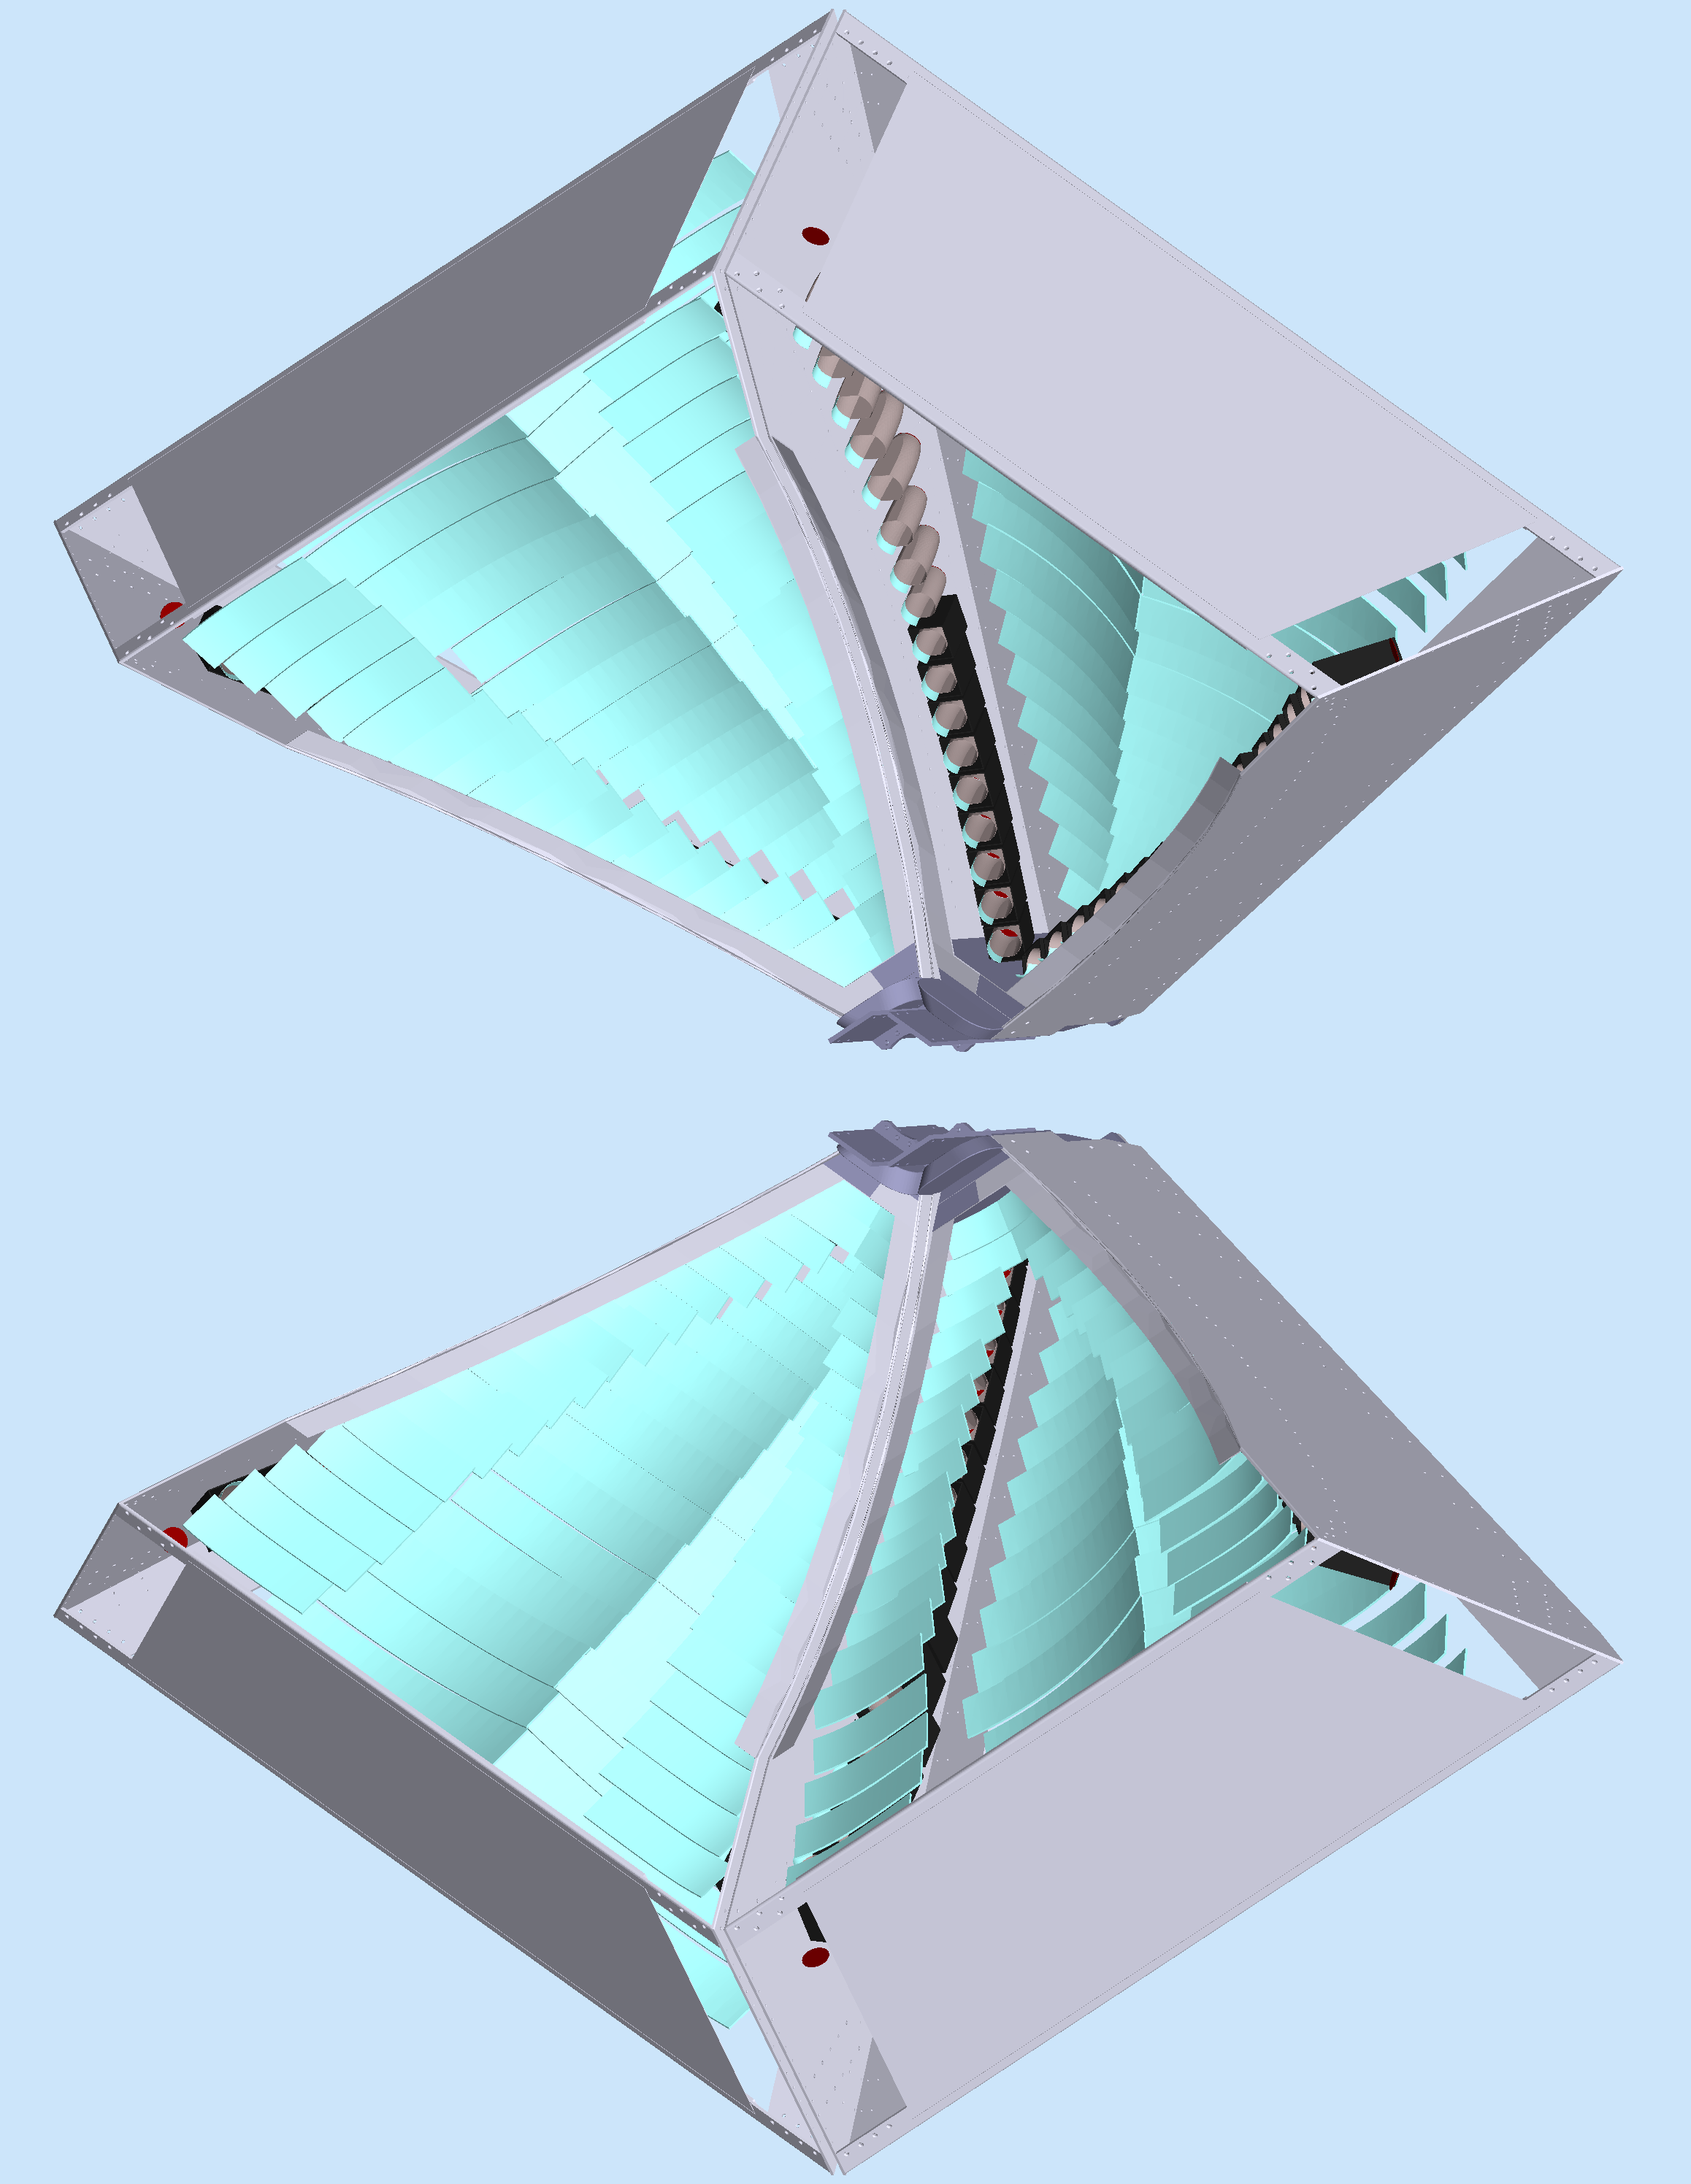
\includegraphics[width=0.95\columnwidth,keepaspectratio]{img/simOverview.png}
	\caption{The geant4 model of the LTCC implemented in GEMC. This view correspond to the Run Group A CLAS12 experiments
				where the LTCC sectors 2, 3, 5 and 6 were present. In this picture the hyperbolic mirrors and some magnetic shields
            in sector3 (upper right) have been made transparent to show details of the Winston Cones (grey) and magnetic shields (black).}
	\label{fig:simOverview}
\end{figure}

\subsection{Geometry}

The Cherenkov light is emitted on a small cone around the direction of the emitting particle. The angle of
incidence of the particles entering the LTCC can be different from the angle at the production vertex due
to the bending of the tracks inside the toroidal magnetic field.
Instead of having two sets of mirrors, one aligned for in-bending (toward the beamline) and one aligned for
out-bending (away from the beamline) particles, the optics of the mirrors was designed to maximize the
light collection of optical photons originating from the target (placed on the center of the CLAS12 coordinate system),
to average the cases for the two charged particles.

The mirror shapes were described mathematically by ellipsoid and hyperbolic curves.
The ellipsoid first focal point is the target location and the second focal point was chosen
to place the mirrors as far back in the box as possible to maximize the amount of gas seen by the tracks.
The second ellipsoid focal point overlaps with the hyperbolic first focal point. The hyperbole shape was optimized to focus the light
collection on PMTs placed on the shadow of the torus magnet coil, near the LTCC box walls, see \F{mirrorMath}.


\begin{figure}
	\centering
	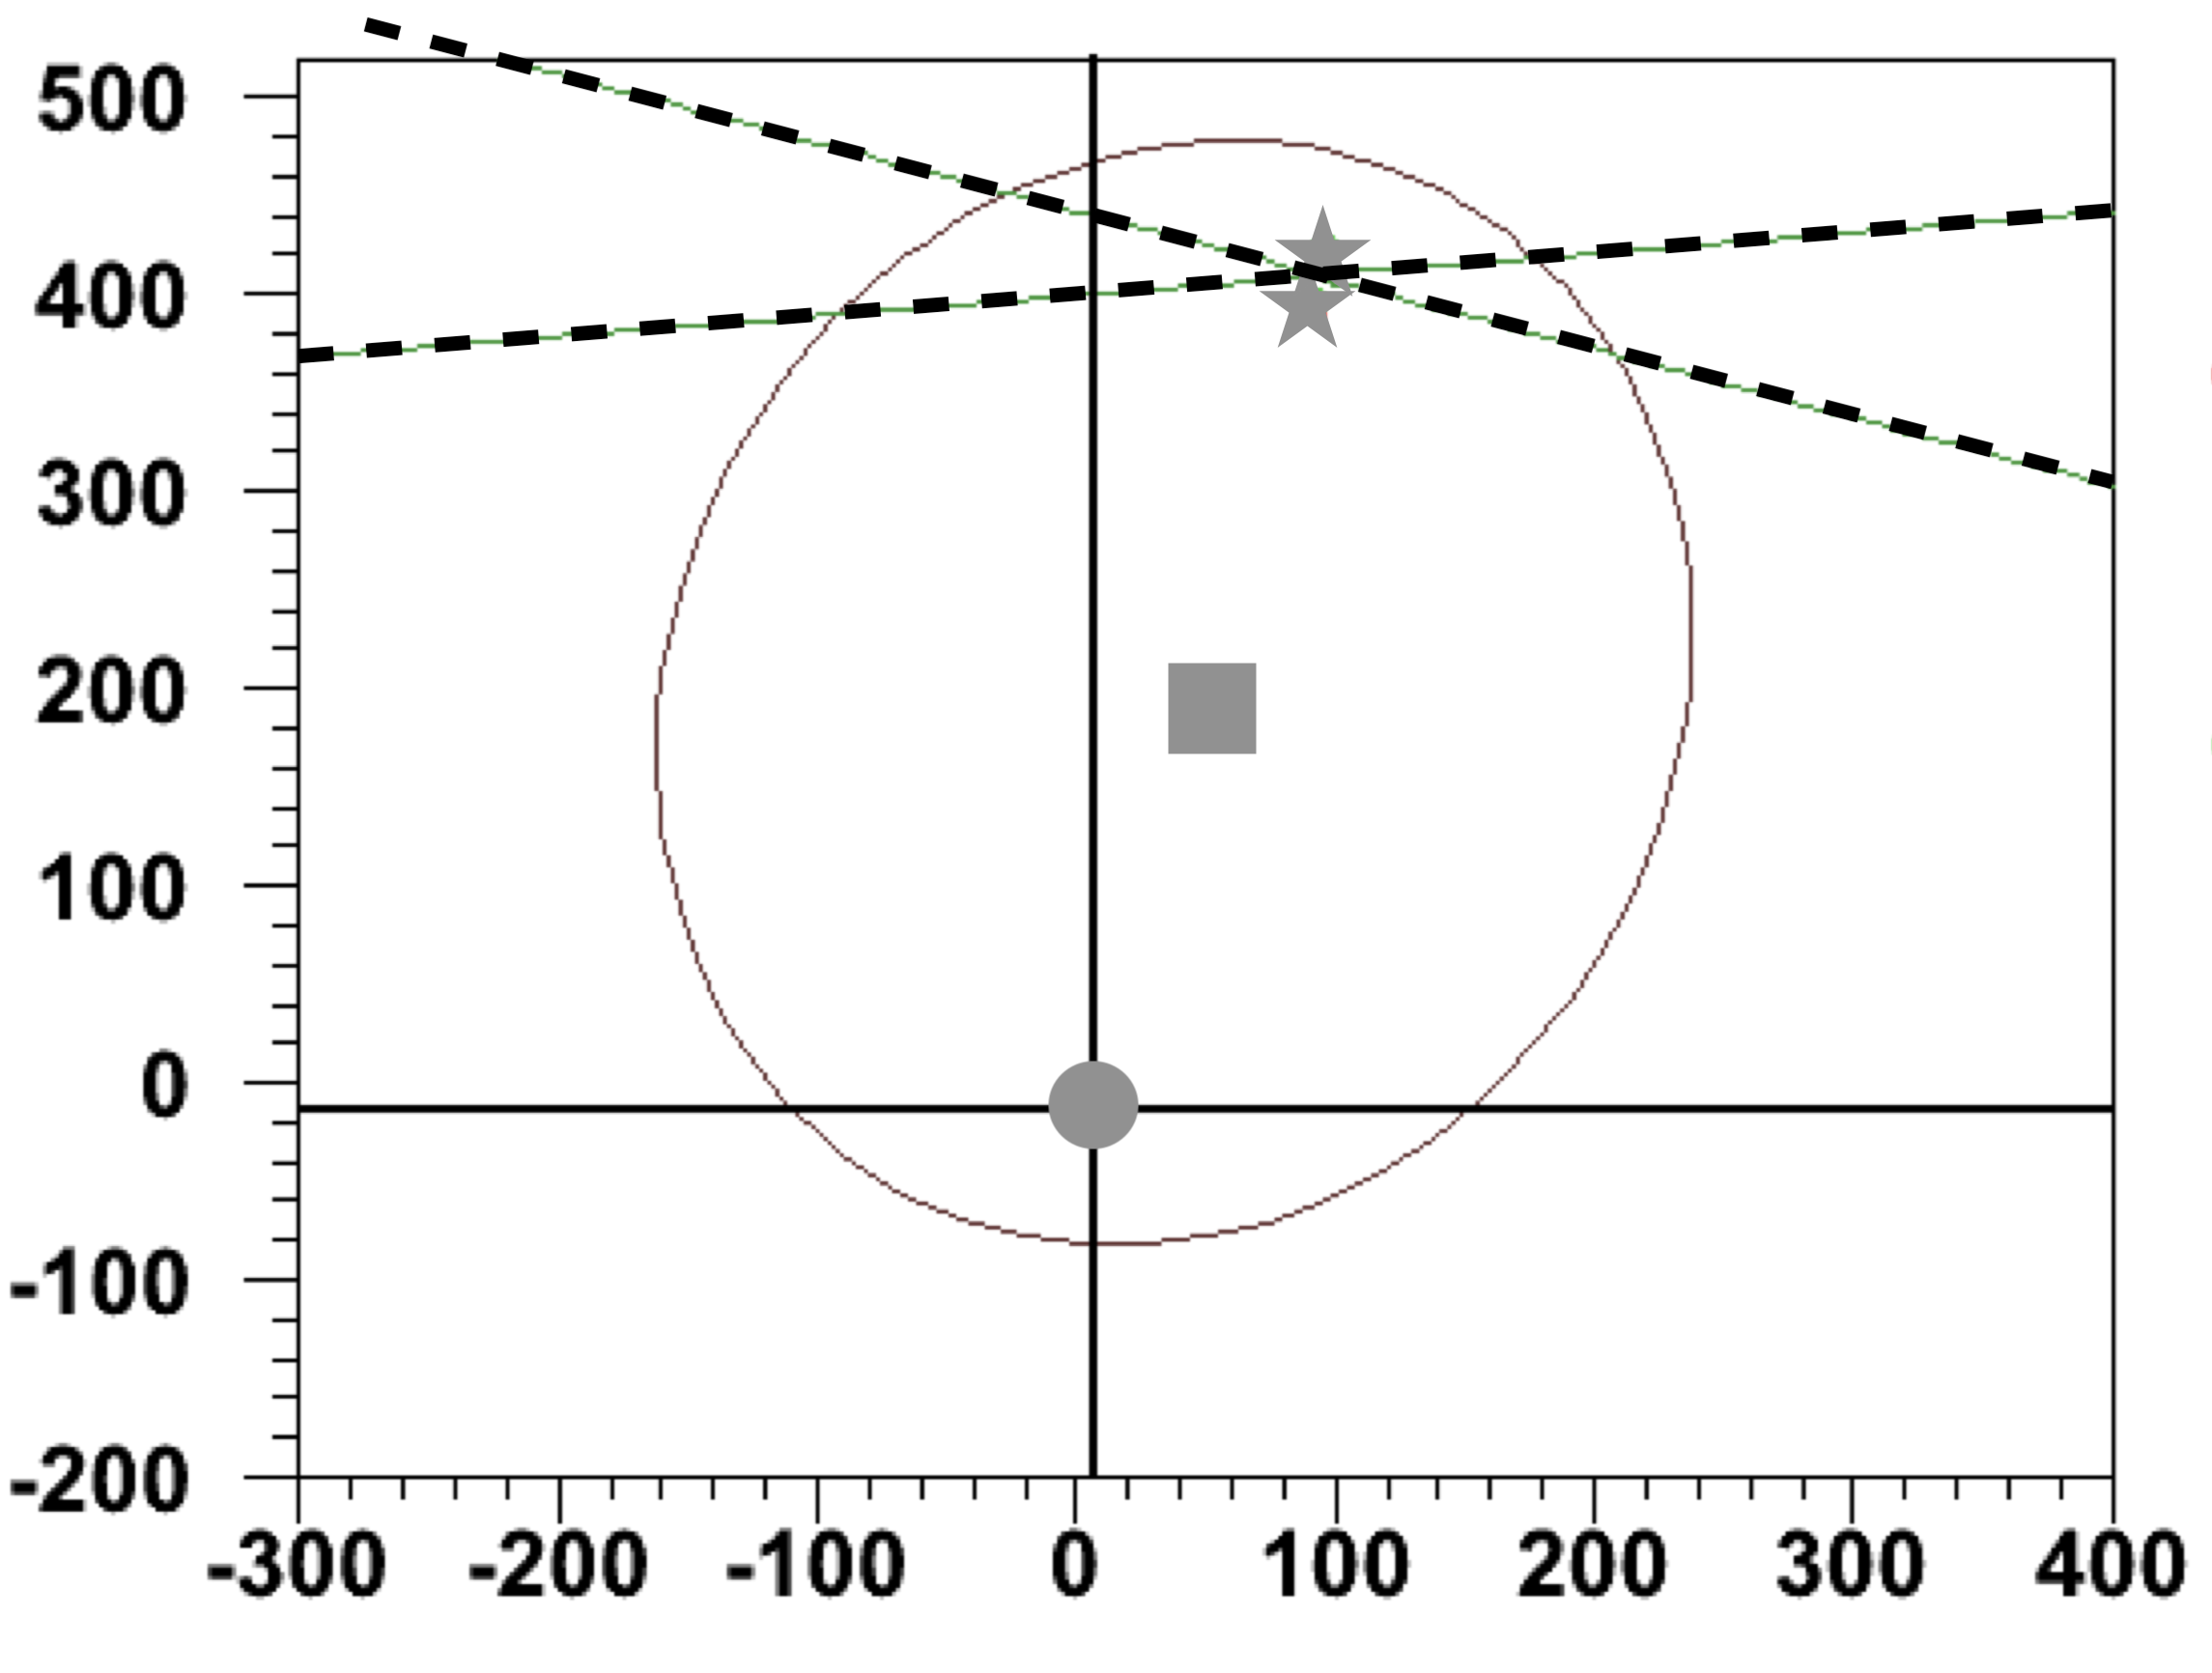
\includegraphics[width=0.95\columnwidth,keepaspectratio]{img/mirrorMath1.png}
	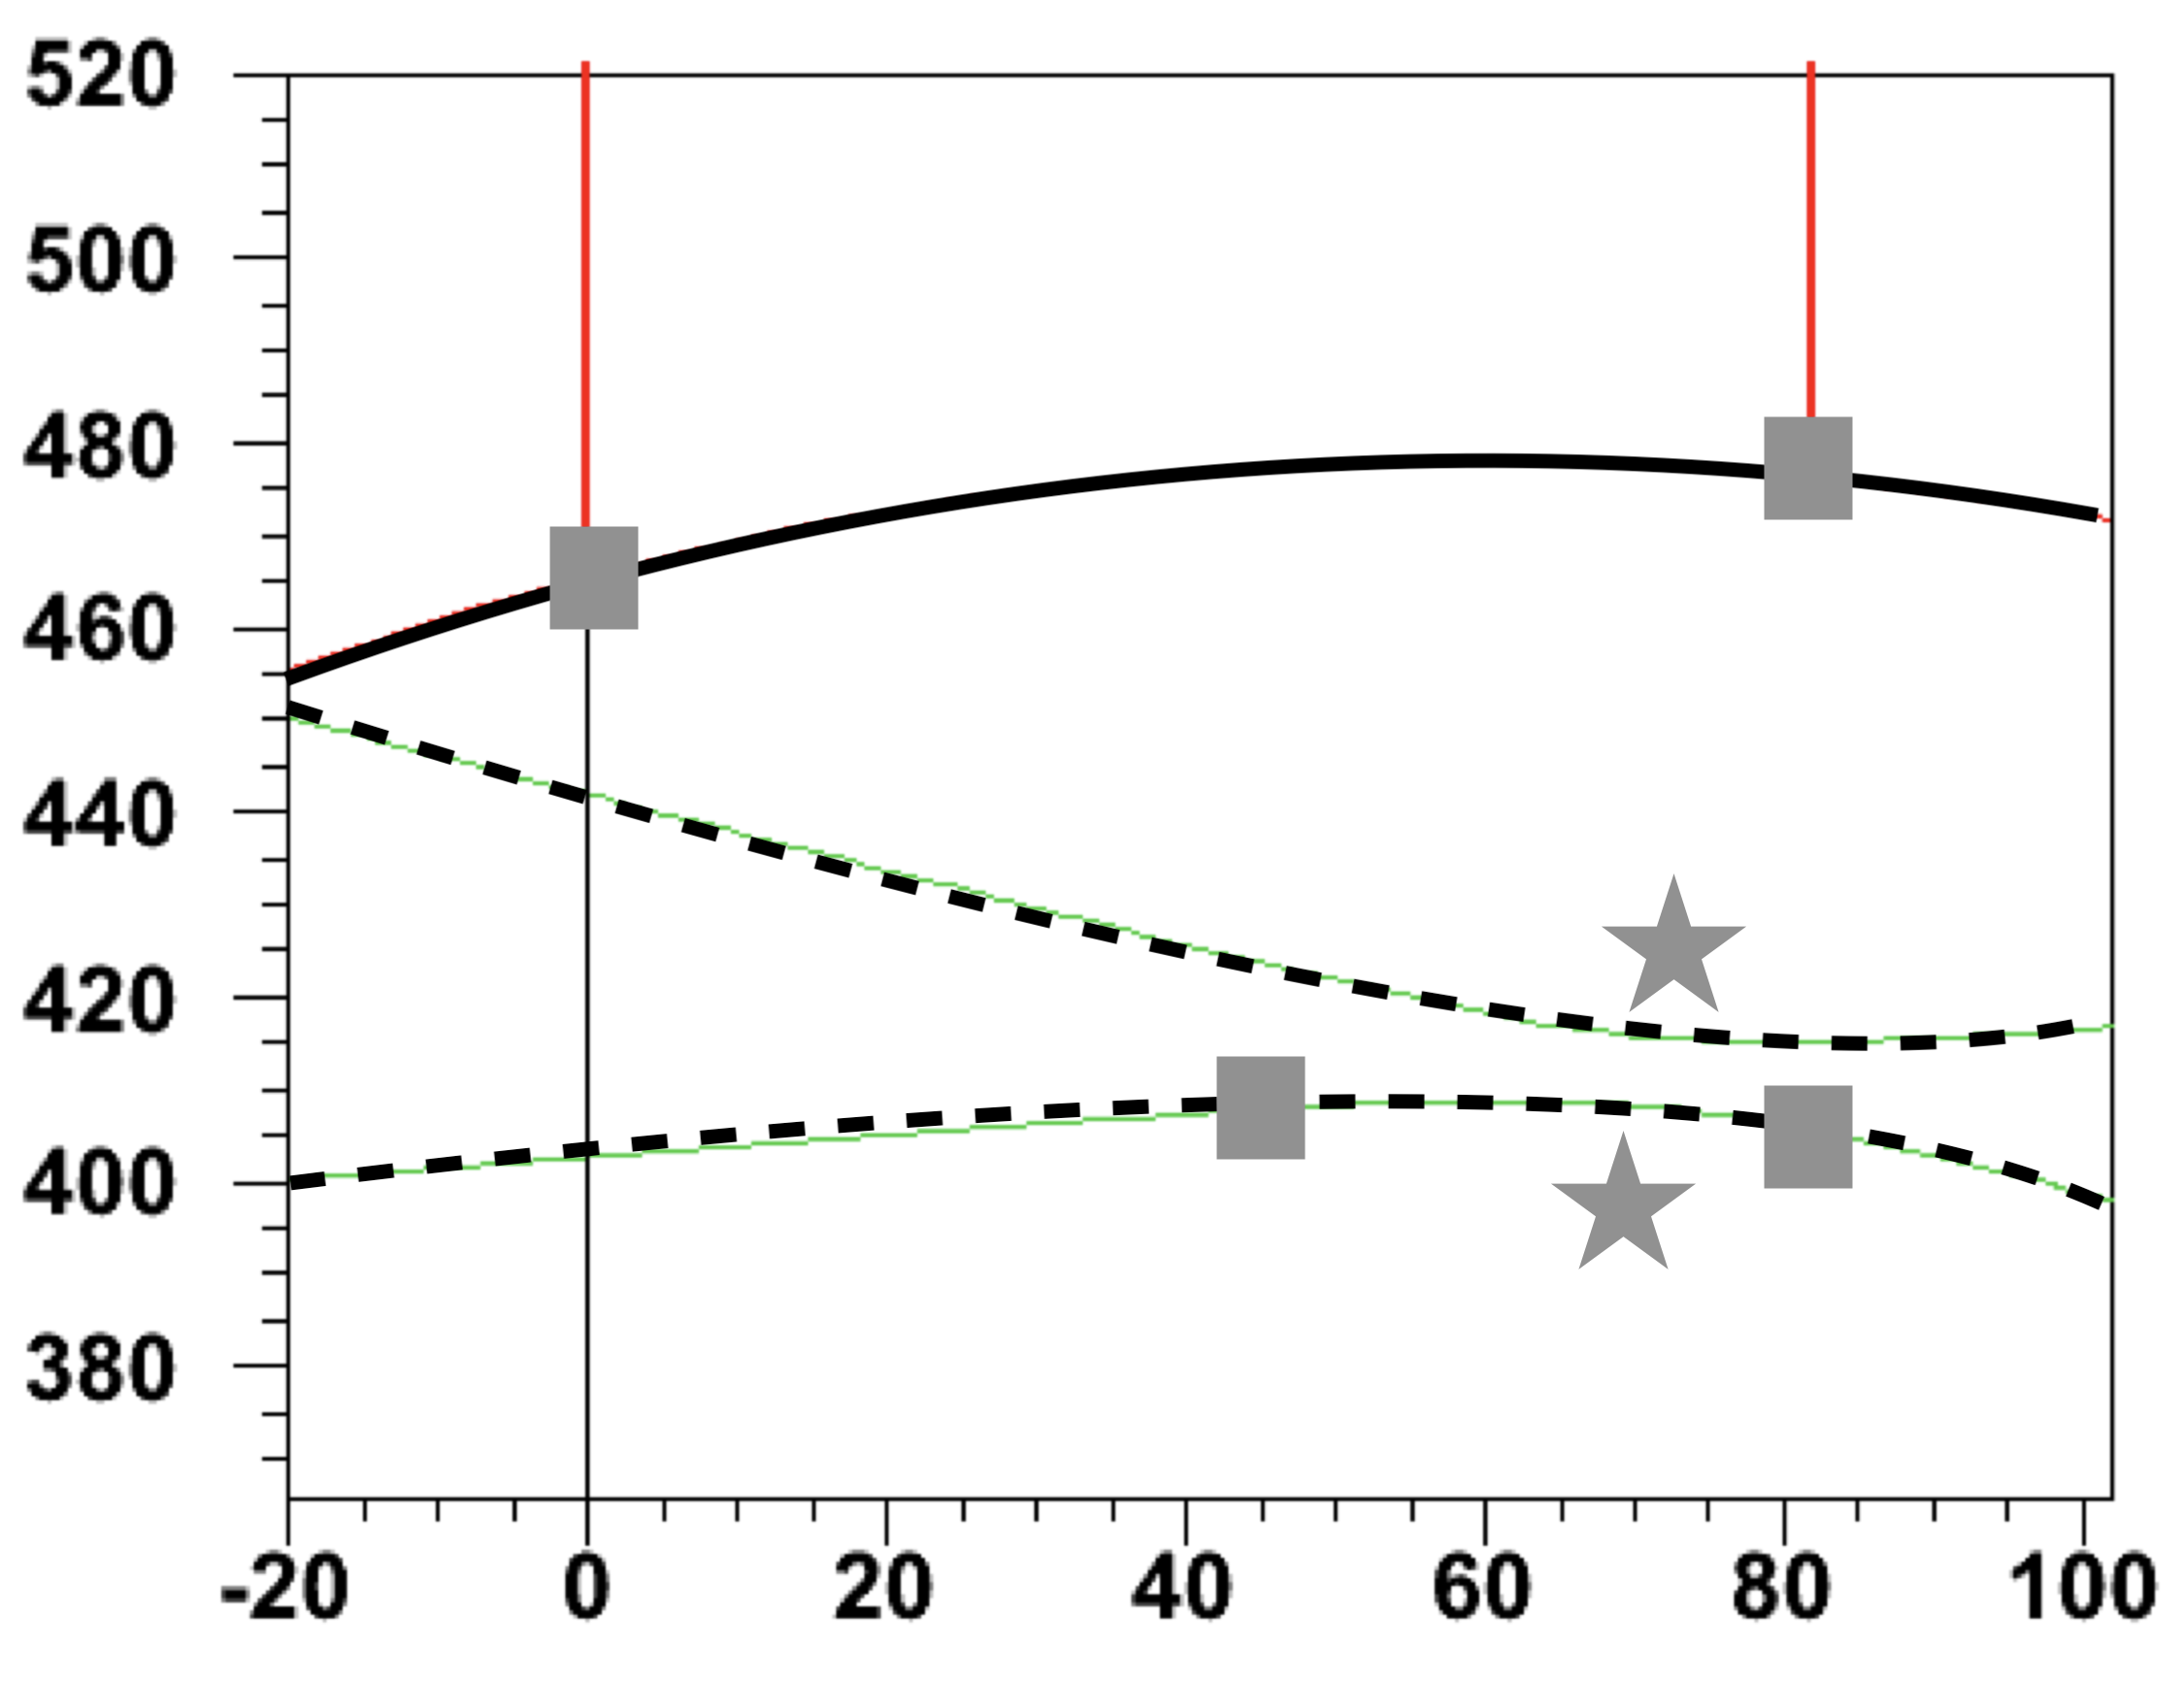
\includegraphics[width=0.95\columnwidth,keepaspectratio]{img/mirrorMath2.png}
	\caption{Top: The ellipsoid shape (black line), with its center (red diamond) and the two focal points (red circles). The two hyperbolas
			   that have the corresponding focal points (green circles) are the green curves. Bottom: details of the mirrors azimuthal limits: the triangles represent
            the elliptical mirror left and right edges. The crosses are the hyperbolic mirrors edges. All these parameters are stored in databases and
            loaded in the software modeling the LTCC mirrors in the GEMC simulation.}
	\label{fig:mirrorMath}
\end{figure}

In the geant4 implementation the elliptical mirrors are composed by, for each segment:

\begin{enumerate}
	\item ellipse shells: the subtraction of two ellipsoidal volumes, rotated and centered on their designed position for the mirrors on the right side of the box.
	\item ellipse azimuthal slices: subtraction of the shells with left and right boxes to ``cut'' the mirrors left and right edges
	\item placed mirrors: the resulting volumes,  are then copied to their left side of the box counterpart.
\end{enumerate}

The hyperbolic mirrors are made by polycon that approximate the mathematical shape of the mirrors using a number of faucets
varying from 10 (smallest mirror) to 30 faucets (longest mirrors). The measured reflectivity is imported in the simulation as
optical property of the mirror material.


The CAD engineering models of the WC have been used in the simulations, see \F{wcSimulation}. The measured reflectivity is imported in the simulation as
optical property of the WC material. The WC and the PMTs volumes are surround by boxes of mu-metal that model the LTCC magnetic shields, see \F{simShield}.

\begin{figure}
	\centering
	\includegraphics[width=0.95\columnwidth,keepaspectratio]{img/wcLargeReal.png}
	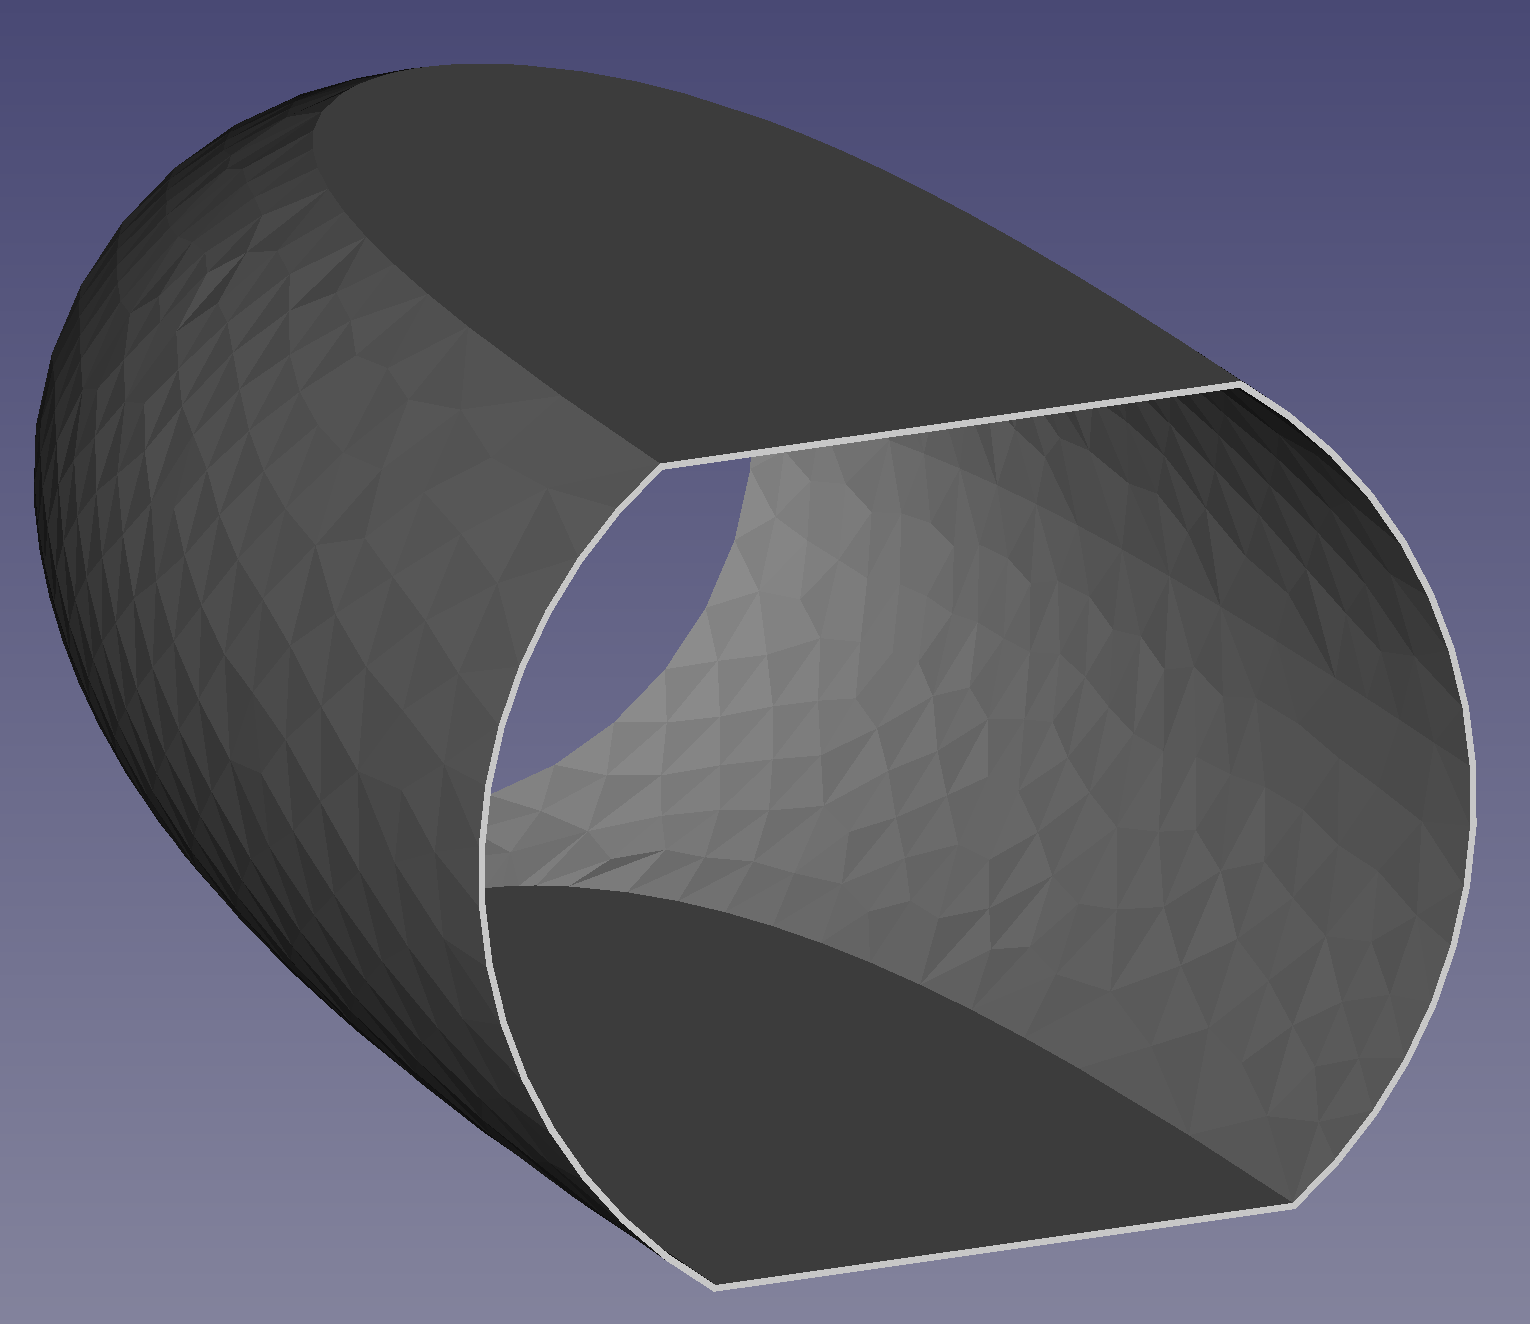
\includegraphics[width=0.95\columnwidth,keepaspectratio]{img/wcLargeSim.png}
	\caption{Top: a picture of the large WC used for segments 12 to 18. Bottom: the tessellated volume used in the
            simulation, imported from the CAD engineering model.}
	\label{fig:wcSimulation}
\end{figure}

\begin{figure}
	\centering
	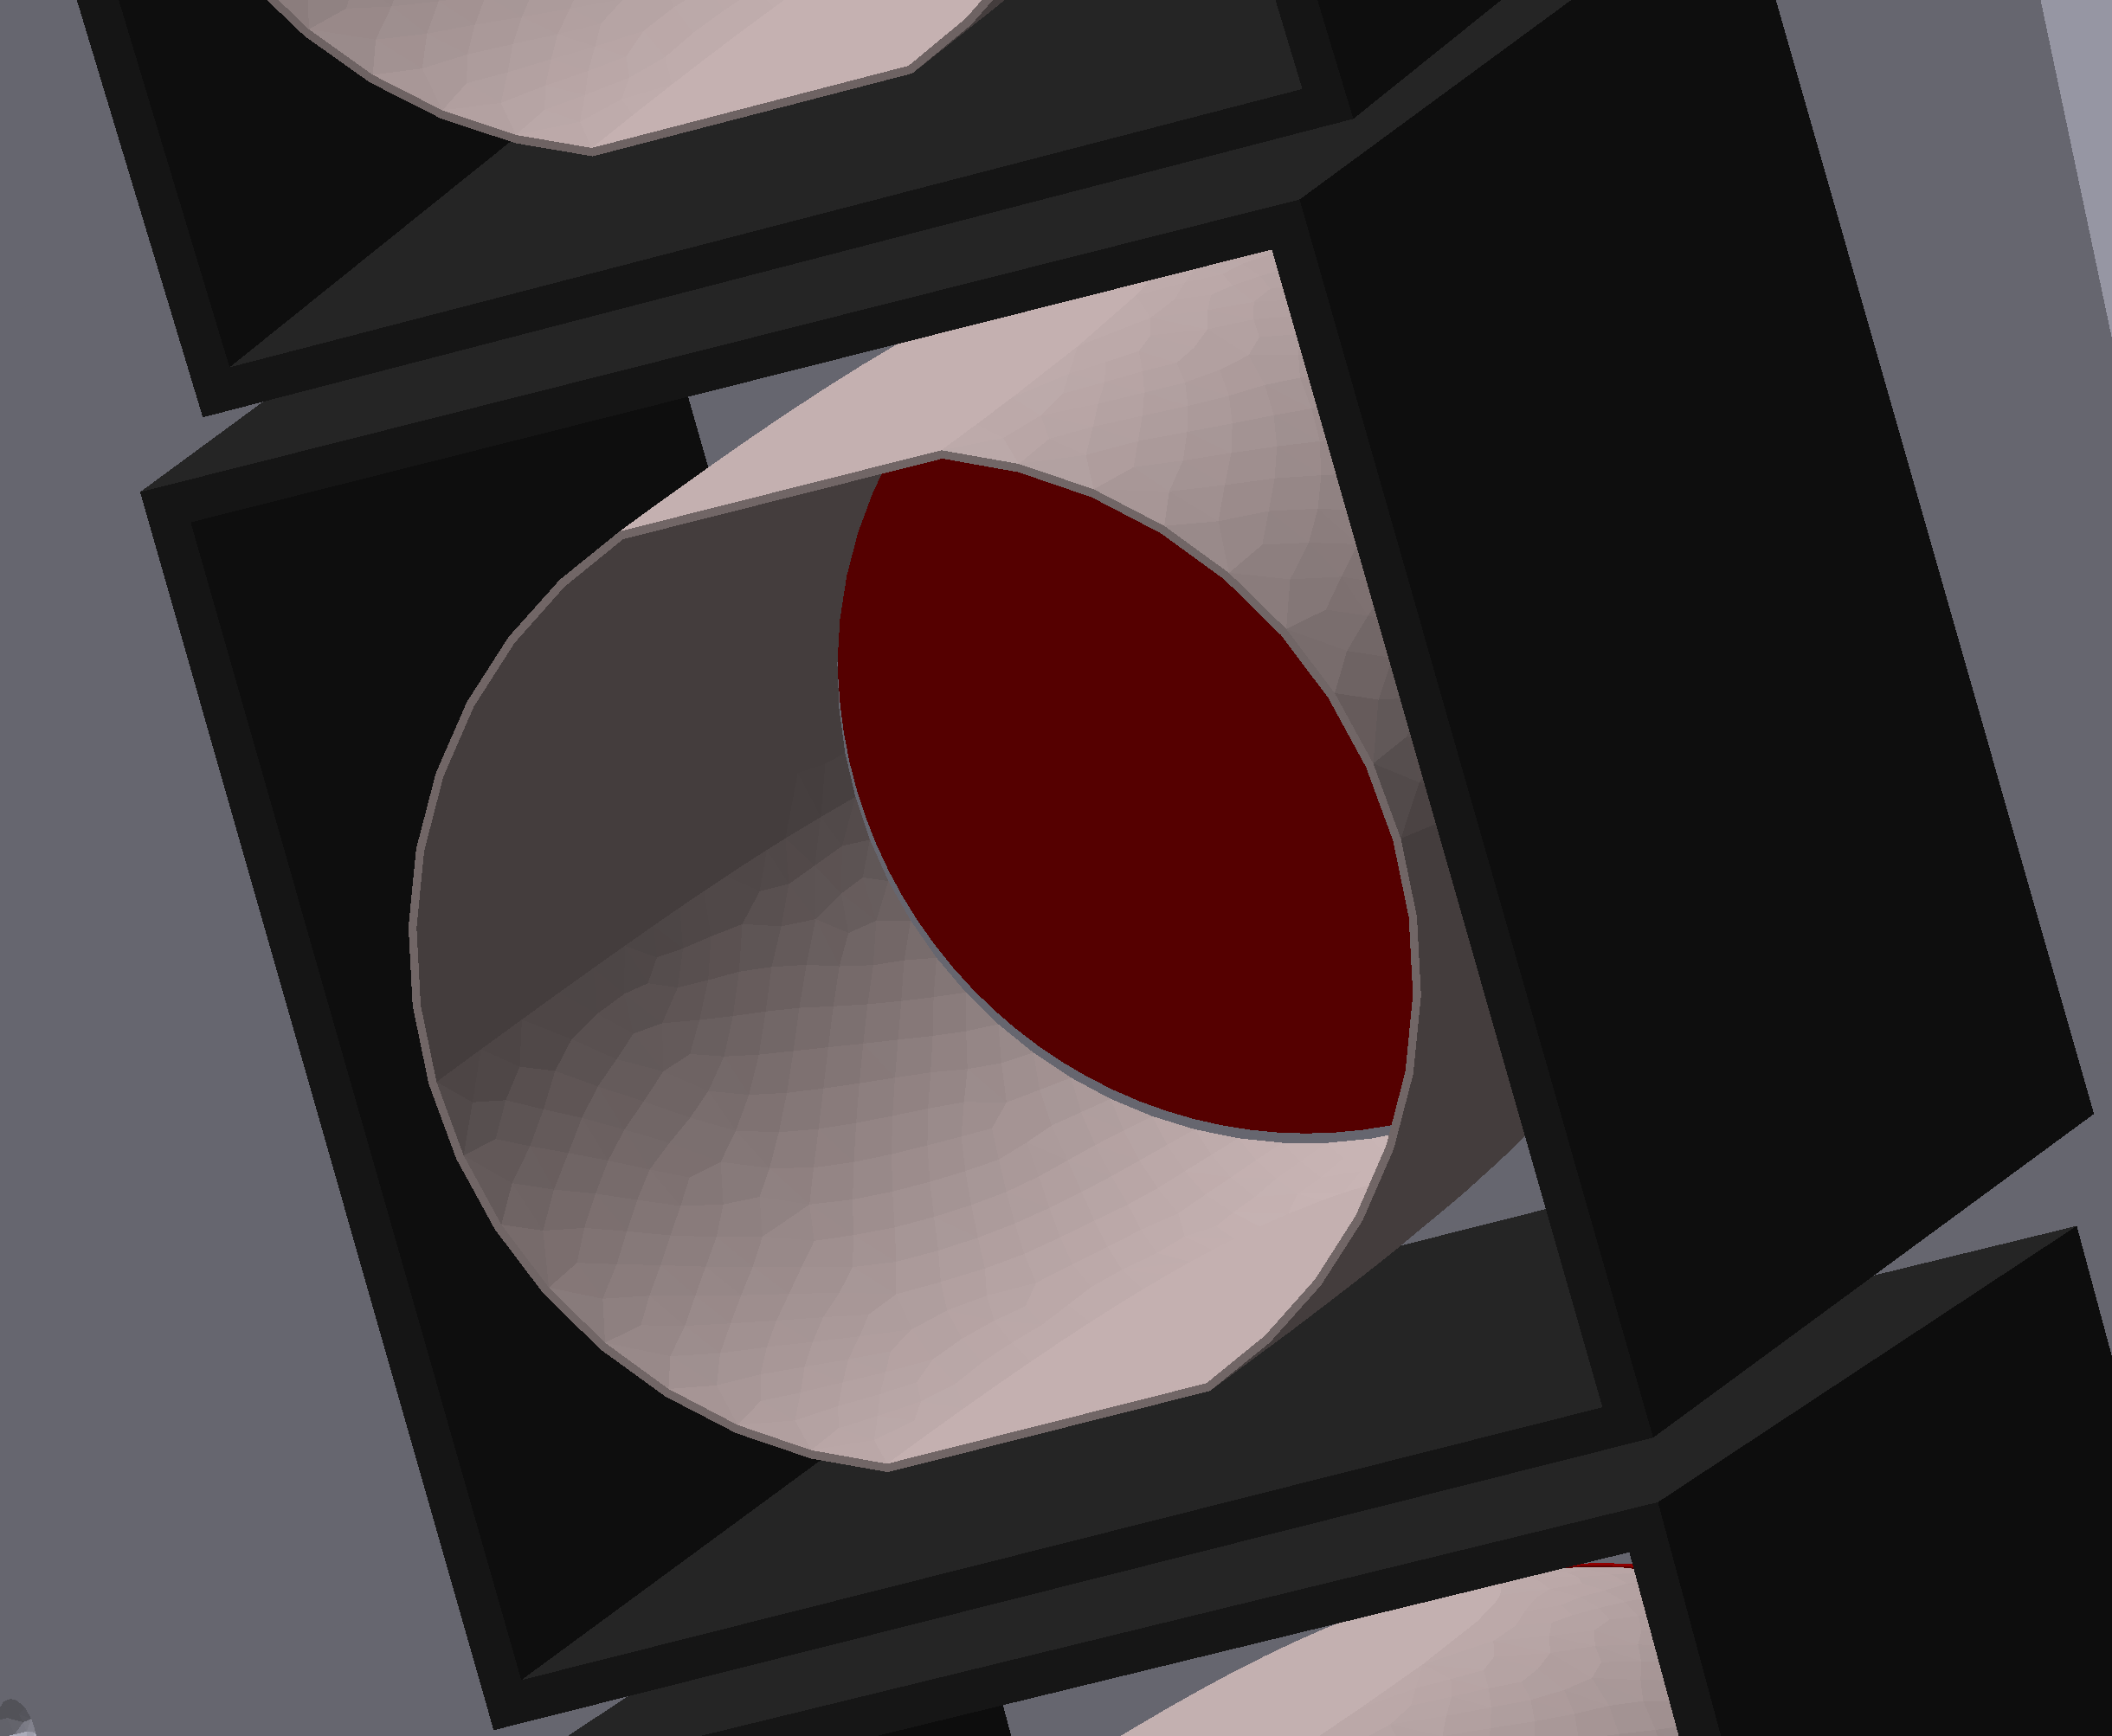
\includegraphics[width=0.95\columnwidth,keepaspectratio]{img/simShield.png}
	\caption{The magnetic shields are modeled by metal boxes in the GEMC simulations (black). The WC (grey) focus the light on the red PMT surface.}
	\label{fig:simShield}
\end{figure}


The LTCC box support structure was imported from the engineering model shown in \F{boxCut}. This includes the 1 cm thick aluminum
elliptical and hyperbolic mirror support flanges, the nose and the hardware mount to the CLAS12 beam line.


\subsection{Digitization}

In the digitization the number of collected photons detected is converted to ADC by taking into account:

\begin{itemize}
	\item The quantum efficiency of the PMTs
	\item The position and width of the single photo-electron peak as stored in the CCDB database after calibration
\end{itemize}


\subsection{Run Period Variations}

As the CLAS12 experiments started, not all sectors could be filled with the the $C_4F_{10}$ gas, thus some sectors where removed from the
forward carriage. As they were installed or removed from the forward carriage, gas leaks were found and fixed. These geometry changes are imported in the simulations as database
variations. The default simulations only includes Sector 2 (S2), S3, S5 and S6 as the RICH detector is replacing S1 and S6.
The variations are listed in Table \ref{tab:simVariations}.

\begin{table}
	\begin{center}
		\begin{tabular}{| l | c |}
			\hline \hline
			Run Period       & Sectors Installed and Gas \\
			\hline
			Default          & S2, S3, S5, S6, all $C_4F_{10}$    \\
			RGA Spring 2018  & S2, S3, S6 (N2), S5 ($C_4F_{10}$)  \\
			RGA Fall 2018    & S3 ($C_4F_{10}$), S5 (N2)          \\
			RGB Spring 2018  & S3 ($C_4F_{10}$), S5 ($C_4F_{10}$) \\
			\hline \hline
		\end{tabular}
	\end{center}
	\caption{LTCC Simulations variations for different run periods. Shown are which sectors are present and the gas in each sector}
	\label{tab:simVariations}
\end{table}






